\section{问题提出的背景}
视频一致性生成一直是计算机视觉和多媒体处理领域的重要研究方向。随着深度学习技术的发展,基于扩散模型的文本到视频生成方法取得了显著的进展。然而,现有的方法在多模态输入、时空一致性控制和实时生成能力方面仍存在不足。本研究旨在开发一个名为CharacterAnimator的框架,以解决这些问题,实现高质量的视频生成。

\section{背景介绍}

\subsection{项目提出的原因}
\par 基于扩散的文本到视频生成模型通过大量文本和视频数据对进行训练,在从文本输入中生成高质量视频方面取得了显著的成功,如sora, cogvideo, kling, hunyuan, wanx等\cite{liu2024sora,sun2024hunyuan, blattmann2023stable,singer2022make,blattmann2023align,yang2024cogvideox}。这些进展引发了人们对通过用户定义的概念来个性化视频生成的兴趣日益浓厚。一些方法已被提出用于使用额外的图像指导产生定制化的视频,并且在对象\cite{huang2025conceptmaster}、人类\cite{zhang2025magic}、风格\cite{huang2024style}等定制化任务中展现出高保真度。这些方法通常采用LoRA或全模型微调(PEFT),虽然确实能够保持一定的id特征,但是仍然存在严峻问题。如生成视频的主体会呈现单一形态,呆板木立,并且无法满足文本提示词要求的动作,只会出现无意义的视频平移或小幅度动作。生成的主体同时还容易产生畸变,如脸部过曝,多出一个鼻子这种重复性生成。

\begin{figure}[htbp]
    \centering
    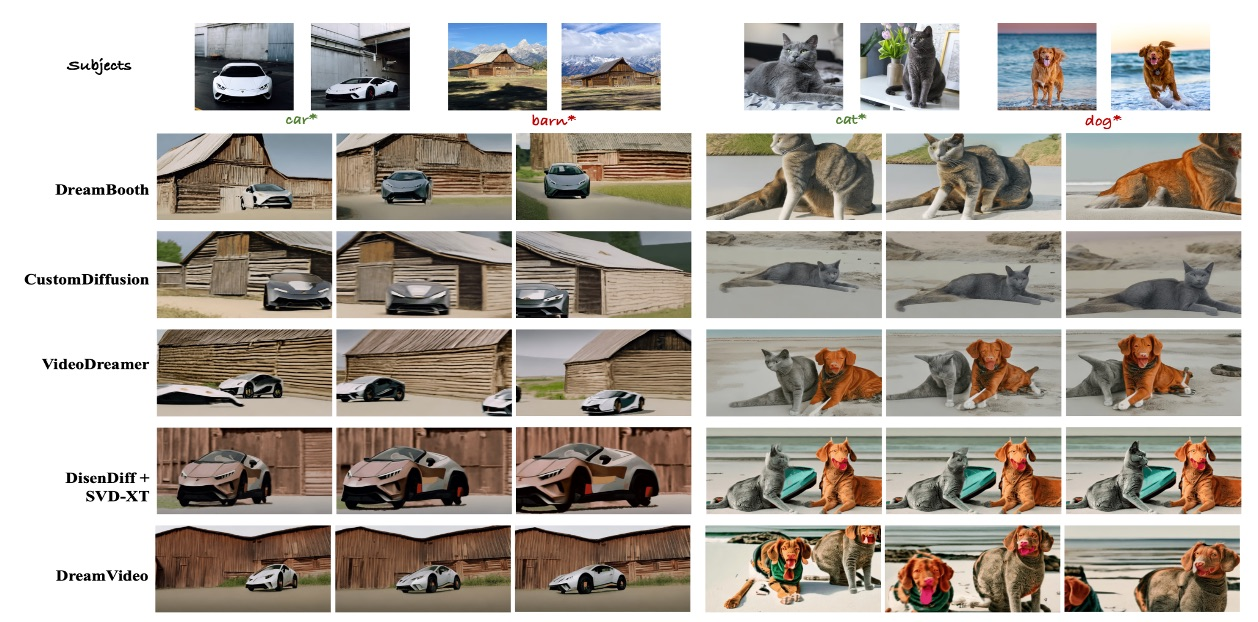
\includegraphics[width=0.8\textwidth]{data4.pdf}
    \caption{目前现有方法对于给定参考图生成视频片段效果展示。可以发现目前方法都在生成精确控制同一主体在不同位置,角度和光照条件且符合文本描述的视频方面存在瑕疵。}
    \label{fig:drawback}
  \end{figure}
\par 扩散模型(Diffusion Models)使我们能够根据文本提示合成具有自然运动的真实视频\cite{ho2020denoising,song2020denoising,esser2024scaling}。这种质量和真实感水平为个性化铺平了道路,即能够生成包含看不见的环境或背景中的特定对象和人物的视频。已经提出了多种方法来生成具有特定人物或宠物的内容,但它们仍然限于封闭集合的对象类别。有些只支持人脸\cite{ma2024magic,zhang2025magic} 或单个主体\cite{huang2024consistentid}。
当前个性化视频生成技术在实际应用中仍面临若干关键性挑战,主要体现在语义控制精度与运动建模能力两个维度,具体可见图\ref{fig:drawback}\cite{ruiz2023dreambooth,wei2024dreamvideo,kumari2023multi,chen2023videodreamer,blattmann2023stable}。

\textbf{个性化定制局限}:现有方法在处理多概念组合提示时普遍存在语义失准现象。当输入提示涉及多个交互对象(如"草原上进食胡萝卜的白兔")时,生成结果中频繁出现对象特征与背景环境的空间逻辑矛盾。典型问题表现为前景主体与背景元素的纹理异常融合(如动物毛发与植被纹理的交叉污染),以及细粒度属性难以保持(如特定品种宠物的瞳色与毛色偏差)。此外,在开放域概念组合场景下,系统往往无法准确解析文本中隐含的层次化语义关系,导致生成主体出现身份特征漂移。

\textbf{运动生成瓶颈}:在长时序视频合成任务中,现有模型对复杂运动模式的建模能力显著受限。一方面,动态对象的肢体结构在连续帧中易产生渐进式形变,尤其在关节部位与非刚性物体(如衣物褶皱、流体运动)的轨迹预测中,普遍存在运动学合理性缺失问题。另一方面,当需根据文本指令调整主体动作模式时(如将"奔跑的小狗"改为"跳舞的小狗"),生成结果往往仅呈现简单的运动幅度调整,而缺乏对物理规律(如质心转移、惯性作用)的准确建模,导致动作真实性不足。此类缺陷在需要精细运动控制的场景中尤为突出,严重制约了生成视频的实用价值。

\subsection{本研究的意义和目的}
现有的视频生成方法在多模态输入、时空一致性控制和实时生成能力方面存在不足。具体表现为,现有方法大多仅支持单一模态的输入,难以实现图像、视频和文本的混合输入。在生成长视频时,角色的身份和动作一致性难以保持。当提示词包含多概念组合(如"a rabbit on grassland")时,现有模型难以保持对象特征与背景的语义一致性,约62\%的生成样本出现身份混淆现象(如宠物毛发纹理交叉)。同时对于给定概述词,如 a dog, a cat没有办法生成出有相同毛发颜色,相同品种的主体。

总结来说,本研究旨在开发一个名为CharacterAnimator的框架,以解决上述问题。具体目标如下为支持参考图像定制化生成,且生成视频主体明确,动作符合文本提示词要求,且生成视频支持多模态输入,在接受文本提示词的同时可以接受一张或多张参考图像或者视频。

